\begin{figure}[h]
\centering
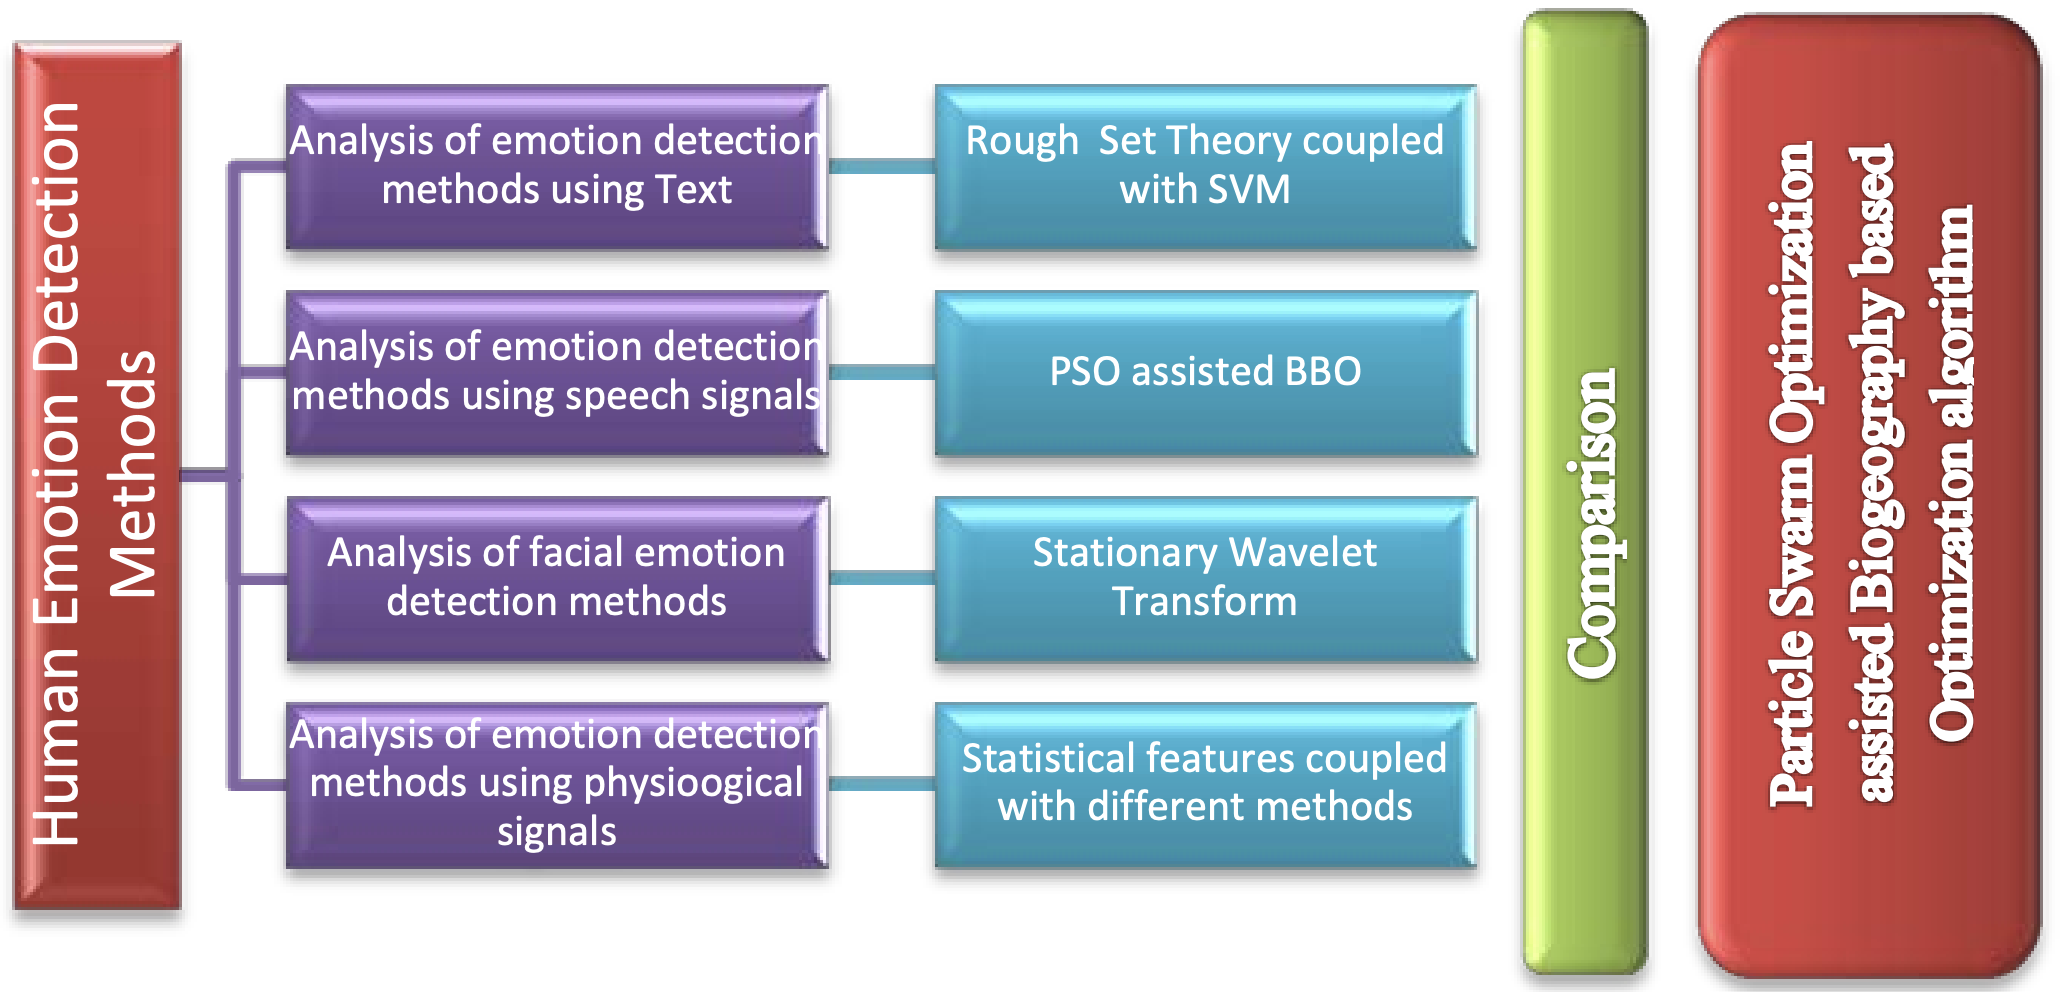
\includegraphics[width=1\textwidth]{images/Emotion-detection-survey.png}
\caption{Survey on Emotional Detection. \cite{EGGER201935}}\label{fig:survey}
\end{figure}

%\noindent The current work on emotional recognition is an active and rapidly developing field with many applications as already touched upon in chapter \ref{chap:introduction}. Like Figure \ref{fig:survey} shows, there are many possibilities to approach this. Continuing, we will focus on \acrshort{fer} and \acrshort{ser}.\\

%\noindent \acrshort{fer} is an important area of research that has many applications in \acrshort{hci} and other fields. \acrfull{cnn} have emerged as a promising approach for \acrshort{fer}, but there are numerous factors that can impact their performance. As of today, there are multiple state-of-the-art \acrshort{cnn}-based \acrshort{fer} methods that differ in their architecture, preprocessing, and training/test protocols, of which Christopher Pramerdorfer and Martin Kampel has analyzed six of in their book: Facial Expression Recognition using Convolutional Neural Networks: State of the Art\cite{pramerdorfer2016facial}.

%\noindent Especially recognizing facial expressions under naturalistic conditions is still an unsolved problem and represents a great challenge. One way to improve \acrshort{fer} performance is to overcome the bottleneck of using comparatively basic CNN architectures. A collection of modern \acrshort{cnn} has achieved a test accuracy of 75.2\% on the FER2013 dataset\cite{FER2013}. Outperforming previous works without requiring auxiliary training data or face registration \cite{pramerdorfer2016facial}.

%\noindent In the area of \acrshort{ser} the research is ongoing. Also, in the specific branch of \acrshort{hci} \acrshort{cnn} are commonly used for feature extraction and classification in \acrshort{ser}. Besides, \acrfull{rnn} (especially Gated Recurrent Unit architectures) are also effective methods for emotion recognition through speech. In this case the highest accuracy scored was 97.47\%. \cite{GRU}.

%\noindent It is also interesting to have a look at the transformer-based models, which recently were used for \acrshort{ser} with promising results \cite{transform}. \acrshort{ser} under realistic conditions presents several challenges, including the variability in speech patterns and background noise.


% NEW VERSION --

\noindent Due to the fact that the current research and development of the emotional recognition is an active and rapidly progressing field in the Human Computer Interaction sector, there are lot of related works and already successfully implemented methods. The positive effects of utilizing these advanced techniques are increasing, with society recognizing the benefits they bring to various sectors such as healthcare and the public sector. \\

\noindent The paper "Emotion Recognition from Physiological Signal Analysis: A Review" \cite{EGGER201935} provides a comprehension of over hundred of papers and a detailed analysis of the methodologies used along with the dataset for facial expression recognition, physiological signals recognition, speech signals variation and text semantics (see Figure \ref{fig:survey}). As a logical consequence we will focus on the \acrshort{fer} and \acrshort{ser} considering six elementary emotions: sadness, surprise, disgust, happiness, fear and anger. \\


\noindent First we will have a look at \acrshort{fer}. is pointing out two main categories of methods - feature based techniques and model based techniques. The highest accuracy was scored with the Stationary Wavelet Transform (see Figure \ref{fig:survey}) for FER with 97.47\%. Besides, the recognition of facial expression under naturalistic condition is still an unsolved problem and represents a great challenge. \\

\noindent Secondly, \acrshort{ser} instead is mainly divided into prosodic features, phonetic features, mathematical models and neural models. Here, underlining 99.47\% were scored with Particle Swarm Optimization assisted Biogeography based optimization algorithms (see Figure \ref{fig:survey}). Furthermore, \acrshort{ser} under realistic conditions presents several challenges, including the variability in speech patterns and background noise. \\
